
\de{ĐỀ THI HỌC KỲ I NĂM HỌC 2022-2023}{Trường THPT Lương Ngọc Nguyên - Thái Nguyên}
\begin{center}
	\textbf{PHẦN 1 - TRẮC NGHIỆM}
\end{center}
\Opensolutionfile{ans}[ans/ans]
%Câu 1...........................
\begin{ex}%[0D1B3-4]%[Dự án đề kiểm tra HKI NH22-23- Võ Thị Thùy Trang]%[Lương Ngọc Quyến - Thái Nguyên]
	Cho các tập hợp $A=\left[-5;\dfrac{1}{2}\right]$, $B=\left(-3;+\infty\right)$. Khi đó tập hợp $A \cap B$ bằng tập hợp nào sau đây?
	\choice
	{$\left\{x \in \mathbb{R}\mid -3\leq x< \dfrac{1}{2}\right\}$}
	{$\left\{x \in \mathbb{R}\mid -5<x\leq \dfrac{1}{2}\right\}$}
	{\True $\left\{x \in \mathbb{R}\mid -3<x\leq \dfrac{1}{2}\right\}$}
	{$\left\{x \in \mathbb{R}\mid -3 \leq x\leq \dfrac{1}{2}\right\}$}
	\loigiai{
		Ta có $A \cap B= \left(-3;\dfrac{1}{2}\right]=\left\{x \in \mathbb{R}\mid -3<x\leq \dfrac{1}{2}\right\}$.
	}
\end{ex}
\begin{ex}%[0H2B3-4]%[Dự án đề kiểm tra HKI NH22-23- Võ Thị Thùy Trang]%[Lương Ngọc Quyến - Thái Nguyên]
	Cho hai vectơ $\overrightarrow{a}$ và $\overrightarrow{b}$ không cùng phương. Hai vectơ nào sau đây cùng phương?	
	\choice
	{$-\dfrac{1}{2}\overrightarrow{a}+\overrightarrow{b}$ và $2\overrightarrow{a}+\overrightarrow{b}$}
	{$-3\overrightarrow{a}+\overrightarrow{b}$ và $-\dfrac{1}{2}\overrightarrow{a}+6\overrightarrow{b}$}
	{\True $\dfrac{1}{2}\overrightarrow{a}-\overrightarrow{b}$ và $-\dfrac{1}{2}\overrightarrow{a}+\overrightarrow{b}$}
	{$\dfrac{1}{2}\overrightarrow{a}+\overrightarrow{b}$ và $\overrightarrow{a}-2\overrightarrow{b}$}
	\loigiai{
		Đặt $\overrightarrow{u}=\dfrac{1}{2}\overrightarrow{a}-\overrightarrow{b}$ và $\overrightarrow{v}=-\dfrac{1}{2}\overrightarrow{a}+\overrightarrow{b}$.\\
		Ta có $\overrightarrow{u}=\dfrac{1}{2}\overrightarrow{a}-\overrightarrow{b}=-\left(-\dfrac{1}{2}\overrightarrow{a}+\overrightarrow{b}\right)=-\overrightarrow{v}$.\\
		Vậy hai vectơ $\dfrac{1}{2}\overrightarrow{a}-\overrightarrow{b}$ và $-\dfrac{1}{2}\overrightarrow{a}+\overrightarrow{b}$ cùng phương. 	
	}
\end{ex}
\begin{ex}%[0X1B3-2]%[Dự án đề kiểm tra HKI NH22-23- Võ Thị Thùy Trang]%[Lương Ngọc Quyến - Thái Nguyên]
	Điểm thi môn Toán cuối năm của một nhóm gồm $7$ học sinh lớp 11 là $1$; $3$; $4$; $5$; $7$; $8$; $9$. Số trung vị của dãy số liệu đã cho là
	\choice
	{$6$}
	{$4$}
	{\True $5$}
	{$7$}
	\loigiai{
		Vì cỡ mẫu bằng $7$ nên trung vị là số liệu thứ $4$ của dãy, tức là $M_{e}=5$.	
	}
\end{ex}
\begin{ex}%[0H2K3-6]%[Dự án đề kiểm tra HKI NH22-23- Võ Thị Thùy Trang]%[Lương Ngọc Quyến - Thái Nguyên]
	Cho hình vuông $ABCD$ cạnh $a$. Khi đó $\left|2\overrightarrow{AD}+\overrightarrow{DB}\right|=?$
	\choice
	{$a$}
	{\True $a\sqrt{2}$}
	{$a\sqrt{3}$}
	{$2a$}
	\loigiai{
		Ta có $2\overrightarrow{AD}+\overrightarrow{DB}=\overrightarrow{AD}+\overrightarrow{AD}+\overrightarrow{DB}=\overrightarrow{AD}+\overrightarrow{AB}=\overrightarrow{AC}$.\\
		Ta suy ra $\left|2\overrightarrow{AD}+\overrightarrow{DB}\right|=\left|\overrightarrow{AC}\right|=AC=a\sqrt{2}$.	
	}
\end{ex}
\begin{ex}%[0X1B4-3]%[Dự án đề kiểm tra HKI NH22-23- Võ Thị Thùy Trang]%[Lương Ngọc Quyến - Thái Nguyên]
	Sĩ số học sinh của $5$ lớp khối $10$ là $40$; $43$; $45$; $41$; $46$. Độ lệch chuẩn của mẫu số liệu trên gần nhất với số nào trong các đáp án sau?
	\choice
	{$2{,}42$}
	{\True $2{,}28$}
	{$2{,}25$}
	{$2{,}52$}
	\loigiai{
		Sĩ số trung bình của $5$ lớp khối 10 là
		$\dfrac{40+43+45+41+46}{5}=43$.\\
		Phương sai của mẫu số liệu là
		$S^2=\dfrac{1}{5}\left(40^2+43^2+45^2+41^2+46^2\right)-43^2=\dfrac{26}{5}$.\\
		Độ lệch chuẩn của mẫu số liệu là
		$S=\sqrt{S^2}=\sqrt{\dfrac{26}{5}} \approx 2{,}28$.			
	}
\end{ex}
\begin{ex}%[0X1B3-1]%[Dự án đề kiểm tra HKI NH22-23- Võ Thị Thùy Trang]%[Lương Ngọc Quyến - Thái Nguyên]
	Số bàn thắng trong các trận của một giải bóng đá được ghi lại như sau
	\begin{center}
		\begin{tabular}{|c|c|c|c|c|c|c|}
			\hline
			Số bàn thắng & 1 & 2 & 3 & 4 & 5 & 6 \\
			\hline
			Số trận đấu & 5 & 14 & 16 & 10 & 3 & 2 \\
			\hline
		\end{tabular}
	\end{center}
	Số bàn thắng trung bình trong một trận của cả giải là
	\choice
	{$2{,}69$}
	{$3{,}69$}
	{\True $2{,}96$}
	{$3{,}96$}
	\loigiai{
		Số bàn thắng trung bình trong một trận của cả giải là\\
		$\overline{x}=\dfrac{1 \cdot 5 + 2 \cdot 14 +3 \cdot 16 +4 \cdot 10 +5 \cdot 3 +6 \cdot 2}{50}=2{,}96$.	
	}
\end{ex}
\begin{ex}%[0X1B3-4]%[Dự án đề kiểm tra HKI NH22-23- Võ Thị Thùy Trang]%[Lương Ngọc Quyến - Thái Nguyên]
	Cho bảng số liệu
	\begin{center}
		\begin{tabular}{|c|c|c|c|c|c|c|}
			\hline
			$x_i $ & 2 & 3 & 4 & 5 & 6 & Cộng \\
			\hline
			$n_i $ & 5 & 15 & 10 & 6 & 7 & 43 \\
			\hline
		\end{tabular}
	\end{center}
	Mốt của bảng số liệu đã cho là
	\choice
	{$5$}
	{\True $3$}
	{$6$}
	{$2$}
	\loigiai{
		Theo số liệu trong bảng thì tần số lớn nhất là $15$ ứng với giá trị là $3$ nên mốt của bảng số liệu đã cho là $3$. 	
	}
\end{ex}
\begin{ex}%[0H2B1-5]%[Dự án đề kiểm tra HKI NH22-23- Võ Thị Thùy Trang]%[Lương Ngọc Quyến - Thái Nguyên]
	Cho tam giác đều $ABC$. Mệnh đề nào sau đây \textbf{sai}?
	\choice
	{$\left|\overrightarrow{AB}\right|=\left|\overrightarrow{BC}\right|$}
	{$\overrightarrow{AC}$ không cùng phương với $\overrightarrow{BC}$}
	{\True $\overrightarrow{AB}=\overrightarrow{BC}$}
	{$\overrightarrow{AC} \neq \overrightarrow{BC}$}
	\loigiai{
		Hai vectơ $\overrightarrow{AB}$ và $\overrightarrow{BC}$ có độ dài bằng nhau nhưng không cùng phương nên hai vectơ này không bằng nhau. 	
	}
\end{ex}
\begin{ex}%[0H2B2-1]%[Dự án đề kiểm tra HKI NH22-23- Võ Thị Thùy Trang]%[Lương Ngọc Quyến - Thái Nguyên]
	Cho các điểm phân biệt $A,B,C$. Đẳng thức nào sau đây đúng?
	\choice
	{\True $\overrightarrow{AB}=\overrightarrow{CB}+\overrightarrow{AC}$}
	{$\overrightarrow{AB}=\overrightarrow{BC}+\overrightarrow{AC}$}
	{$\overrightarrow{AB}=\overrightarrow{BC}+\overrightarrow{CA}$}
	{$\overrightarrow{AB}=\overrightarrow{CA}+\overrightarrow{BC}$}
	\loigiai{
		Ta có: $\overrightarrow{CB}+\overrightarrow{AC}=\overrightarrow{AC}+\overrightarrow{CB}=\overrightarrow{AB}$.	
	}
\end{ex}
\begin{ex}%[0X1B1-1]%[Dự án đề kiểm tra HKI NH22-23- Võ Thị Thùy Trang]%[Lương Ngọc Quyến - Thái Nguyên]
	Cho giá trị gần đúng của $\dfrac{8}{17}$ là $0{,}47$. Sai số tuyệt đối của $0,47$ không vượt quá
	\choice
	{$0{,}0003$}
	{\True $0{,}0006$}
	{$0{,}0004$}
	{$0{,}0002$}
	\loigiai{
		Gọi $\overline{a}=\dfrac{8}{17}$ và $a=0{,}47$.\\
		Sai số tuyệt đối là\\
		$\Delta _{a}=\left|\overline{a}-a\right|=\left|\dfrac{8}{17}-0{,}47\right| \approx 0{,}00058 \leq 0{,}0006$.	
	}
\end{ex}
\begin{ex}%[0D1B3-4]%[Dự án đề kiểm tra HKI NH22-23- Võ Thị Thùy Trang]%[Lương Ngọc Quyến - Thái Nguyên]%[Câu 11] 
	Cho hai tập hợp $A=\left\{x\in \mathbb{R}|x+3<4+2x\right\}$ và $B=\left\{x\in \mathbb{R}|5x-3<4x-1\right\}$. Có bao nhiêu số tự nhiên thuộc tập $A\cap B$?
	\choice
	{\True $2$}
	{$1$}
	{$3$}
	{$0$}
	\loigiai{
		Ta có $x+3<4+2x\Leftrightarrow x>-1\Rightarrow A=\left(-1;+\infty\right)$.\\
		$5x-3<4x-1\Leftrightarrow x<2\Rightarrow B=\left(-\infty;2\right)$.
		Do đó $A\cap B=\left(-1;2\right)$.\\
		Vậy có $2$ số tự nhiên thuộc tập $A\cap B$ là $0$; $1$.}
\end{ex}
\begin{ex}%[0H2K3-3]%[Dự án đề kiểm tra HKI NH22-23- Võ Thị Thùy Trang]%[Lương Ngọc Quyến - Thái Nguyên]%[Câu 12]
	Đẳng thức nào sau đây mô tả đúng hình vẽ bên dưới?
	\begin{center}
		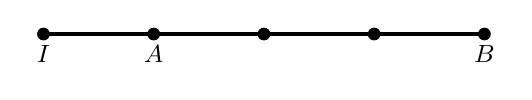
\begin{tikzpicture}[>=stealth,scale=0.7, line join=round, line cap=round]
			%\draw[line width=0.07pt,dashed] (-0.5,-0.5) grid (8.5,2.5);
			\draw[fill=black] (-1,1) circle(3pt) (1,1) circle(3pt) (3,1) circle(3pt) (5,1) circle(3pt) (7,1) circle(3pt);
			\draw[line width = 1.4pt] (-1,1)node[below]{\small$I$}--(1,1)node[below]{\small$A$}--(5,1)--(7,1) node[below]{\small$B$};
		\end{tikzpicture}
	\end{center}
	\choice
	{$3\overrightarrow{IA}+\overrightarrow{IB}=\overrightarrow{0}$}
	{\True $3\overrightarrow{AI}+\overrightarrow{AB}=\overrightarrow{0}$}
	{$\overrightarrow{AI}+3\overrightarrow{AB}=\overrightarrow{0}$}
	{$\overrightarrow{BI}+3\overrightarrow{BA}=\overrightarrow{0}$}
	\loigiai{
		\begin{center}
			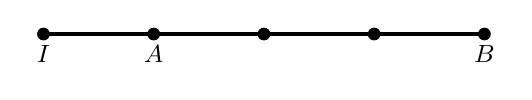
\begin{tikzpicture}[>=stealth,scale=0.7, line join=round, line cap=round]
				%\draw[line width=0.07pt,dashed] (-0.5,-0.5) grid (8.5,2.5);
				\draw[fill=black] (-1,1) circle(3pt) (1,1) circle(3pt) (3,1) circle(3pt) (5,1) circle(3pt) (7,1) circle(3pt);
				\draw[line width = 1.4pt] (-1,1)node[below]{\small$I$}--(1,1)node[below]{\small$A$}--(5,1)--(7,1) node[below]{\small$B$};
			\end{tikzpicture}
		\end{center}
		Theo hình vẽ ta có $3\overrightarrow{AI}+\overrightarrow{AB}=\overrightarrow{0}$}
\end{ex}
\begin{ex}%[0H2B2-5]%[Dự án đề kiểm tra HKI NH22-23- Võ Thị Thùy Trang]%[Lương Ngọc Quyến - Thái Nguyên]%[Câu 13]
	Cho tam giác đều $ABC$ cạnh $a$, trọng tâm là $G$. Phát biển nào là đúng?
	\choice
	{$\overrightarrow{GA}=\overrightarrow{GB}=\overrightarrow{GC}$}
	{$\overrightarrow{AB}=\overrightarrow{AC}$}
	{\True $\left| \overrightarrow{AB}+\overrightarrow{AC}\right|=\sqrt{3}\left| \overrightarrow{AB}-\overrightarrow{AC}\right|$}
	{$\left| \overrightarrow{AB}+\overrightarrow{AC}\right|=2a$}
	\loigiai{
		\begin{center}
			\begin{tikzpicture}[smooth,font=\footnotesize,scale=0.6]
				\path
				(0,0) coordinate (B)
				(4,0) coordinate (C)
				($(B)!1!60:(C)$)coordinate (A)
				($(B)!0.5!(C)$)coordinate (M);
				\draw (A)--(B)--(C)--cycle (A)--(M);
				\foreach \x/\g in {A/90,B/-90,C/-90,M/-90} \draw [fill=black] (\x) circle (.05) + (\g:.4) node{$\x$};
			\end{tikzpicture}
		\end{center}
		Gọi $M$ là trung điểm của $BC$.
		\begin{itemize}
			\item [$\bullet$] Ta có $\vec{AB}-\vec{AC}=\vec{CB}$ nên $\left| \vec{AB}-\vec{AC} \right|=CB=a$.
			\item [$\bullet$] Ta có $\vec{AB}+\vec{AC}=\vec{AD}$ với $D$ là đỉnh thứ 4 của hình bình hành $ABDC$.\\ Suy ra  $\left| \vec{AB}+\vec{AC} \right|=AD=2AM=a\sqrt{3}$.
			\item Vậy	$\left| \overrightarrow{AB}+\overrightarrow{AC}\right|=\sqrt{3}\left| \overrightarrow{AB}-\overrightarrow{AC}\right|$.
		\end{itemize}
	}
\end{ex}
\begin{ex}%[0X1B4-1]%[Dự án đề kiểm tra HKI NH22-23- Võ Thị Thùy Trang]%[Lương Ngọc Quyến - Thái Nguyên]%[Câu 14]
	Cho dãy số liệu thống kê
	$11$; $13$; $14$; $15$; $12$; $10$;  $16$.
	Khoảng tứ phân vị của mẫu số liệu là
	\choice
	{$2$}
	{$10$}
	{\True $4$}
	{$16$}
	\loigiai{
		Sắp xếp lại mẫu số liệu theo thứ tự không giảm, ta được $10$; $11$; $12$; $13$; $14$; $15$; $16$.
		\begin{itemize}
			\item [$\bullet$] Vì cỡ mẫu là $n=7$ là số lẻ nên giá trị tứ phân vị thứ hai là $Q_2=13$.
			\item [$\bullet$] Tứ phân vị thứ nhất là trung vị của mẫu $10; 11; 12$. Do đó $Q_1=11$.
			\item [$\bullet$] Tứ phân vị thứ ba là trung vị của mẫu $14; 15; 16$. Do đó $Q_3=15$.\\
			Vậy khoảng tứ phân vị của mẫu số liệu là $\Delta_Q=Q_3-Q_1=4$.
		\end{itemize}
	}
\end{ex}
\begin{ex}%[0H2B1-4]%[Dự án đề kiểm tra HKI NH22-23- Võ Thị Thùy Trang]%[Lương Ngọc Quyến - Thái Nguyên]%[Câu 15]
	Cho hình bình hành $ABCD$, với giao điểm hai đường chéo là $I$. Khi đó
	\choice
	{\True $\overrightarrow{AB}+\overrightarrow{CD}=\overrightarrow{0}$}
	{$\overrightarrow{AB}+\overrightarrow{IA}=\overrightarrow{BI}$}
	{$\overrightarrow{AB}+\overrightarrow{AD}=\overrightarrow{BD}$}
	{$\overrightarrow{AB}+\overrightarrow{BD}=\overrightarrow{0}$}
	\loigiai{
		\begin{center}
			\begin{tikzpicture}[scale=1, line join=round, line cap=round]
				\tkzDefPoints{0/0/A,4/0/B,5/2/C}
				\tkzDefPointBy[translation=from B to C](A)\tkzGetPoint{D}
				\tkzInterLL(A,C)(B,D)\tkzGetPoint{I}
				\tkzDrawSegments(A,B B,C C,D D,A A,C B,D)
				\tkzDrawPoints[size=2,fill=black](A,B,C,D,I)
				\tkzLabelPoints[below,font=\footnotesize](A, B, I)
				\tkzLabelPoints[above,font=\footnotesize](C,D)
				;
			\end{tikzpicture}
		\end{center}
		Vì $ABCD$ là hình bình hành nên $\overrightarrow{AB}$ và $\overrightarrow{CD}$ là hai vectơ đối nhau. Do đó $\overrightarrow{AB}+\overrightarrow{CD}=\overrightarrow{0}$}
\end{ex}
\begin{ex}%[0D2Y2-1]%[Dự án đề kiểm tra HKI NH22-23- Võ Thị Thùy Trang]%[Lương Ngọc Quyến - Thái Nguyên]%[Câu 16]
	Trong các hệ sau, hệ nào \textbf{không phải} là hệ bất phương trình bậc nhất hai ẩn?
	\choice
	{$\heva{&y>0 \\&x-4\le 1}$}
	{\True $\heva{&x+y=-2 \\&x-y=5}$}
	{$\heva{&x+y>0 \\&x>1}$}
	{$\heva{&x+3y>10 \\&x-4y<1}$}
	\loigiai{
		Hệ $\heva{&x+y=-2 \\&x-y=5}$ không phải là hệ bất phương trình bậc nhất hai ẩn. Đây là hệ phương trình bậc nhất hai ẩn.}
\end{ex}
\begin{ex}%[0X1B4-1]%[Dự án đề kiểm tra HKI NH22-23- Võ Thị Thùy Trang]%[Lương Ngọc Quyến - Thái Nguyên]%[Câu 17]
	Khoảng biến thiên, khoảng tứ phân vị của mẫu số liệu $6; 8; 3; 4; 5; 6; 7; 2; 4$ lần lượt là
	\choice
	{$5$ và $1$}
	{$5$ và $3$}
	{$6$ và $1$}
	{\True $6$ và $3$}
	\loigiai{
		Khoảng biến thiên của mẫu số liệu là $R=8-2=6$.\\
		Sắp xếp lại mẫu số liệu theo thứ tự không giảm, ta được 
		\begin{center}
			$2 \quad 3 \quad 4 \quad 4 \quad 5 \quad 6 \quad 6 \quad 7 \quad 8$.
		\end{center}
		\begin{itemize}
			\item [$\bullet$] Vì cỡ mẫu là $n=9$ là số lẻ nên giá trị tứ phân vị thứ hai là $Q_2=5$.
			\item [$\bullet$] Tứ phân vị thứ nhất là trung vị của mẫu $2; 3; 4; 4$. Do đó $Q_1=3{,}5$.
			\item [$\bullet$] Tứ phân vị thứ ba là trung vị của mẫu $6; 6; 7; 8$. Do đó $Q_3=6{,}5$.\\
			Vậy khoảng tứ phân vị của mẫu số liệu là $\Delta_Q=Q_3-Q_1=3$.
		\end{itemize}
	}
\end{ex}
\begin{ex}%[0H2Y1-4]%[Dự án đề kiểm tra HKI NH22-23- Võ Thị Thùy Trang]%[Lương Ngọc Quyến - Thái Nguyên]%[Câu 18]
	Hai vectơ có cùng độ dài và ngược hướng gọi là
	\choice
	{hai vectơ bằng nhau}
	{\True hai vectơ đối nhau}
	{hai vectơ cùng hướng}
	{hai vectơ có giá trùng nhau}
	\loigiai{
		Hai vectơ có cùng độ dài và ngược hướng gọi là hai vectơ đối nhau.}
\end{ex}
\begin{ex}%[0D2B2-2]%[Dự án đề kiểm tra HKI NH22-23- Võ Thị Thùy Trang]%[Lương Ngọc Quyến - Thái Nguyên]%[Câu 19]
	\immini{Trong hình vẽ dưới đây, phần mặt phẳng không bị gạch (kể cả bờ) biểu diễn miền nghiệm của hệ bất phương trình nào sau đây?
		\choice
		{\True $\heva{&x-2y\le 0 \\&x+3y\ge -2}$}
		{$\heva{&x-2y\ge 0 \\&x+3y\ge -2}$}
		{$\heva{&x-2y<0 \\&x+3y>-2}$}
		{$\heva{&x-2y\le 0 \\&x+3y\le -2}$}}
	{	\begin{tikzpicture}[scale=0.7,>=stealth, font=\footnotesize, line join=round, line cap=round]
			\def\xmin{-5} \def\xmax{4.5}
			\def\ymin{-4} \def\ymax{2.0}
			%\draw[color=gray!50,dashed] (\xmin,\ymin) grid (\xmax,\ymax);	
			\draw[->] (\xmin,0)--(\xmax,0) node [below]{$x$};
			\draw[->] (0,\ymin)--(0,\ymax) node [left]{$y$};
			\fill (0,0) circle (1pt) node[shift={(-135:3mm)}]{$O$};
			\clip (\xmin+0.1,\ymin+0.1) rectangle (\xmax-0.1,\ymax-0.1);
			\draw[smooth,samples=300] plot(\x,{1/2*(\x)});
			\fill[pattern=north east lines,pattern color=blue,opacity=.7]plot[domain=\xmax:\xmin](\x,{1/2*(\x)})--plot[domain=\xmin:\xmax](\x,{\ymin})--cycle;
			\draw[dashed] (2,0)--(2,1)--(0,1);
			\fill (0,1) circle (1pt) node[shift={(180:3mm)}]{$1$};
			\fill (2,0) circle (1pt) node[shift={(-90:3mm)}]{$2$};
			\draw[smooth,samples=300] plot(\x,{-1/3*(\x+2)});
			\fill[pattern=north east lines,pattern color=blue,opacity=.7]plot[domain=\xmax:\xmin](\x,{-1/3*(\x+2)})--plot[domain=\xmin:\xmax](\x,{\ymin})--cycle;
			\fill (0,-0.666) circle (1pt) node[shift={(-130:3mm)}]{\tiny{$-\dfrac{2}{3}$}};
			\fill (-2,0) circle (1pt) node[shift={(90:3mm)}]{$-2$};
			\node at (-3.0,.65)[above]{$x+3y+2=0$};
			\node at (2.0,1.2)[above]{$x-2y=0$};
	\end{tikzpicture}}
	\loigiai{
		Lấy điểm $M(0;1)$ ta thấy $M(0;1)$ thoả cả hai bất phương trình $x-2y\le 0$ và $x+3y\ge -2$.
		Do đó trong hình vẽ trên, phần mặt phẳng không bị gạch (kể cả bờ) biểu diễn miền nghiệm của hệ bất phương trình $\heva{&x-2y\le 0 \\&x+3y\ge -2.}$}
\end{ex}
\begin{ex}%[0H2Y1-3]%[Dự án đề kiểm tra HKI NH22-23- Võ Thị Thùy Trang]%[Lương Ngọc Quyến - Thái Nguyên]%[Câu 20]
	Hai vectơ được gọi là bằng nhau nếu chúng
	\choice
	{cùng hướng}
	{cùng phương}
	{\True cùng hướng và cùng độ dài}
	{có độ dài bằng nhau}
	\loigiai{
		Hai vectơ được gọi là bằng nhau nếu chúng cùng hướng và cùng độ dài}
\end{ex}
		\begin{ex}%[0X1B1-3]%[Dự án đề kiểm tra HKI NH22-23- Võ Thị Thùy Trang]%[Lương Ngọc Quyến - Thái Nguyên]
		Cho số gần đúng $a=23748023$ với độ chính xác $d=101$. Số quy tròn của số $a$ là
		\choice
		{\True $23748000$}
		{$23746000$}
		{$23749000$}
		{$23747000$}
		\loigiai{Do độ chính xác $d=101$ nên số quy tròn của số $a$ là $23748000$.
		}
	\end{ex}
\begin{ex}%[0X1B4-3]%[Dự án đề kiểm tra HKI NH22-23- Võ Thị Thùy Trang]%[Lương Ngọc Quyến - Thái Nguyên]
	Kết quả thi học kì I của bạn A được ghi lại trong bảng sau
	\begin{center}
		\begin{tabular}{|c|c|c|c|c|c|}
			\hline Toán & Văn & Anh & Lý & Hóa & Địa \\
			\hline 7{,}0 & 6{,}0 & 7{,}5 & 7{,}5 & 8{,}5 & 8{,}0 \\
			\hline
		\end{tabular}
	\end{center}
		Phương sai của mẫu số liệu trên gần nhất với kết quả nào sau đây?
	\choice
	{$0{,}35$}
	{$0{,}52$}
	{$0{,}55$}
	{\True $0{,}6$}
	\loigiai{
		Ta có $\overline{x}=\dfrac{7{,}0+6{,}0+7{,}5+7{,}5+8{,}5+8{,}0}{6}=\dfrac{89}{12}$.\\
		Phương sai
		$S^2=\dfrac{1}{6}\left(7{,}0^2+6{,}0^2+2\cdot 7{,}5^2+8{,}5^2+8{,}0^2\right)-\left(\dfrac{89}{12}\right)^2\approx 0{,}618$.\\
	}
\end{ex}
	\begin{ex}%[0H2B3-2]%[Dự án đề kiểm tra HKI NH22-23- Võ Thị Thùy Trang]%[Lương Ngọc Quyến - Thái Nguyên]
		Cho tam giác $ABC$ có $D$ là trung điểm của $AB$, $M$ là trung điểm $CD$. Đẳng thức nào sau đây đúng?
		\choice
		{$\overrightarrow{MC}+\overrightarrow{MA}+2\overrightarrow{BM}=\overrightarrow{0}$}
		{$\overrightarrow{MA}+\overrightarrow{MB}+\overrightarrow{MC}+\overrightarrow{MD}=\overrightarrow{0}$}
		{\True $\overrightarrow{MA}+\overrightarrow{MB}+2\overrightarrow{MC}=\overrightarrow{0}$}
		{$\overrightarrow{MC}+\overrightarrow{MA}+\overrightarrow{MB}=\overrightarrow{0}$}
		\loigiai{
			\immini{ $\overrightarrow{MA}+\overrightarrow{MB}+2\overrightarrow{MC}=2\overrightarrow{MD}+2\overrightarrow{MC}=2\left(\overrightarrow{MD}+\overrightarrow{MC}\right)=\overrightarrow{0}$.
			}
		{\begin{tikzpicture}[scale=0.8,>=stealth, font=\footnotesize, line join=round, line cap=round]
				\coordinate[label=above:$A$] (A) at (0,4);
				\coordinate[label=below:$B$] (B) at (-2,2);
				\coordinate[label=below:$C$] (C) at (4,2);
				\coordinate[label=left:$D$] (D) at ($(A)!0.5!(B)$);
				\coordinate[label=above:$M$] (M) at ($(C)!0.5!(D)$);
				\draw (A)--(B)--(C)--(A) (C)--(D);
				\foreach \diem in {A,B,C,M,D}	\fill (\diem)circle(1.5pt);
		\end{tikzpicture}}
		}
	\end{ex}
\begin{ex}%[0H2B3-1]%[Dự án đề kiểm tra HKI NH22-23- Võ Thị Thùy Trang]%[Lương Ngọc Quyến - Thái Nguyên]
	Cho tam giác $ABC$ với trung tuyến $AM$ và trọng tâm $G$. Khi đó $\overrightarrow{GA}=?$
	\choice
	{$\dfrac{1}{2}\overrightarrow{AM}$}
	{$\dfrac{2}{3}\overrightarrow{GM}$}
	{\True $-\dfrac{2}{3}\overrightarrow{AM}$}
	{$2\overrightarrow{GM}$}
	\loigiai{
		\immini{Ta có $\overrightarrow{GA}=-\dfrac{2}{3}\overrightarrow{AM}$.
		}
	{\begin{tikzpicture}[scale=0.8,>=stealth, font=\footnotesize, line join=round, line cap=round]
			\coordinate[label=above:$A$] (A) at (0,4);
			\coordinate[label=below:$B$] (B) at (-2,2);
			\coordinate[label=below:$C$] (C) at (4,2);
			\coordinate[label=below:$M$] (M) at ($(C)!0.5!(B)$);
			\coordinate[label=left:$G$] (G) at ($(M)!1/3!(A)$);
			\draw (A)--(B)--(C)--(A)--(M);
			\foreach \diem in {A,B,C,M,G}	\fill (\diem)circle(1.5pt);
	\end{tikzpicture}}
	}
\end{ex}
\begin{ex}%[0X1B3-4]%[Dự án đề kiểm tra HKI NH22-23- Võ Thị Thùy Trang]%[Lương Ngọc Quyến - Thái Nguyên]
	Điều tra về số con của $15$ hộ gia đình trong một tổ dân số, với mẫu số liệu như sau
	\begin{center}
		$\begin{array}{llllllllllllllll}2 & 4 & 3 & 2 & 0 & 2 & 2 & 3 & 5 & 1 & 1 & 1 & 4 & 2 & 2.\end{array}$
	\end{center}
	  Mốt của mẫu số liệu trên là
	\choice
	{\True $2$}
	{$0$}
	{$1$}
	{$3$}
	\loigiai{Mốt của mẫu số liệu trên là $2$ vì giá trị $2$ có tần số lớn nhất.
	}
\end{ex}	
\begin{ex}%[0X1B3-3]%[Dự án đề kiểm tra HKI NH22-23- Võ Thị Thùy Trang]%[Lương Ngọc Quyến - Thái Nguyên]
	Tứ phân vị của mẫu số liệu $21$; $35$; $17$; $43$; $8$; $59$; $72$; $119$ là
	\choice
	{\True $Q_1=19,~ Q_2=39,~ Q_3=65{,}5$}
	{$Q_1=65{,}5,~ Q_2=39,~ Q_3=19$}
	{$Q_1=19,~ Q_2=65{,}5,~ Q_3=19$}
	{$Q_1=39,~ Q_2=19,~ Q_3=65{,}5$}
	\loigiai{Sắp xếp mẫu số liệu theo thứ tự không giảm, ta được
		\begin{center}
			$8$; $17$; $21$; $35$; $43$; $59$; $72$; $119$.
		\end{center}
		Khi đó ta xác định được\\ $Q_1=M_e=\dfrac{1}{2}\left(17+21\right)=19,~ Q_2=M_e=\dfrac{1}{2}\left(35+43\right)=39,~ Q_3=M_e=\dfrac{1}{2}\left(59+72\right)=65{,}5$.
	}
\end{ex}
	\begin{ex}%[0X1B4-3]%[Dự án đề kiểm tra HKI NH22-23- Võ Thị Thùy Trang]%[Lương Ngọc Quyến - Thái Nguyên]
		Cho dãy số liệu thống kê
		\begin{center}
		$\begin{array}{llllllll}1 & 2 & 3 & 4 & 5 & 6 &7.\end{array}$
		\end{center}
		Phương sai của mẫu số liệu thống kê đã cho là
		\choice
		{\True $4$}
		{$3$}
		{$1$}
		{$2$}
		\loigiai{Ta có $\overline{x}=\dfrac{1+2+3+4+5+6+7}{7}=4$.\\
			Phương sai $S^2=\dfrac{1}{7}\left[\left(1-4\right)^2+\left(2-4\right)^2+\left(3-4\right)^2+\left(4-4\right)^2+\left(5-4\right)^2+\left(6-4\right)^2+\left(7-4\right)^2\right]=4$.
		}
	\end{ex}
	\begin{ex}%[0X1B4-2]%[Dự án đề kiểm tra HKI NH22-23- Võ Thị Thùy Trang]%[Lương Ngọc Quyến - Thái Nguyên]
		Giá trị bất thường của mẫu số liệu: $4$; $4$; $4$; $4$; $5$; $20$. là
		\choice
		{\True $20$}
		{$4{,}5$}
		{$5$}
		{$4$}
		\loigiai{
			Sắp xếp mẫu số liệu theo thứ tự không giảm, ta được
			\begin{center}
				$4$; $4$; $4$; $4$; $5$; $20$.
			\end{center}
			Khi đó ta xác định được\\ $Q_1=M_e=4,~ Q_2=M_e=\dfrac{1}{2}\left(4+4\right)=4,~ Q_3=M_e=5$.\\
			$\Delta_Q=Q_3-Q_1=5-4=1$.\\
			$Q_3+1{,}5\Delta_Q=6{,}5$; $Q_1-1{,}5\Delta_Q=2{,}5$.\\
			Suy ra giá trị bất thường là $20$.
			
		}
	\end{ex}
\begin{ex}%[0D1B1-3]%[Dự án đề kiểm tra HKI NH22-23- Võ Thị Thùy Trang]%[Lương Ngọc Quyến - Thái Nguyên]
	Mệnh đề phủ định của mệnh đề \lq\lq$\exists x\in\mathbb{R}, 5 x-3x^2=1$\rq\rq ~là
	\choice
	{\lq\lq$\exists x \in \mathbb{R}, 5x-3x^2\geq 1$\rq\rq}
	{\True \lq\lq $\forall x \in \mathbb{R}, 5x-3x^2 \neq 1$\rq\rq}
	{\lq\lq $\exists x \in \mathbb{R}, 5x-3x^2 \neq 1$ \rq\rq}
	{\lq\lq$\forall x \in \mathbb{R}, 5x-3x^2=1$\rq\rq}
	\loigiai{Mệnh đề phủ định của mệnh đề \lq\lq$\exists x\in\mathbb{R}, 5 x-3x^2=1$\rq\rq ~là \lq\lq $\forall x \in \mathbb{R}, 5x-3x^2 \neq 1$\rq\rq.
	}
\end{ex}
	\begin{ex}%[0X1Y4-3]%[Dự án đề kiểm tra HKI NH22-23- Võ Thị Thùy Trang]%[Lương Ngọc Quyến - Thái Nguyên]
		Trong một mẫu số liệu, phương sai bằng
		\choice
		{\True bình phương của độ lệch chuẩn}
		{một nửa của độ lệch chuẩn}
		{căn bậc hai của độ lệch chuẩn}
		{hai lần của độ lệch chuẩn}
		\loigiai{Trong một mẫu số liệu, phương sai bằng bình phương của độ lệch chuẩn.
		}
	\end{ex}
\begin{ex}%[0X1B4-1]%[Dự án đề kiểm tra HKI NH22-23- Võ Thị Thùy Trang]%[Lương Ngọc Quyến - Thái Nguyên]
	Khoảng biến thiên của mẫu số liệu $1$; $2$; $3$; $4$; $5$; $6$; $7$; $8$ là
	\choice
	{\True $7$}
	{$4{,}5$}
	{$2$}
	{$8$}
	\loigiai{Khoảng biến thiên của mẫu số liệu là $R=8-1=7$.
	}
\end{ex}
\begin{ex}%[0D2B1-2]%[Dự án đề kiểm tra HKI NH22-23- Võ Thị Thùy Trang]%[Lương Ngọc Quyến - Thái Nguyên]
	\immini{
	Trong hình vẽ dưới đây, phần mặt phẳng không bị gạch sọc (không kể bờ) biểu diễn miền nghiệm của bất phương trình nào sau đây?
	\choice
	{$2x-y+1>0$}
	{$x+2y-2 \geq 0$}
	{$x+2y+1 \leq 0$}
	{\True $x+2y-2>0$}}
	{\begin{tikzpicture}[scale=0.8,>=stealth, font=\footnotesize, line join=round, line cap=round]
			\def\xmin{-2} \def\xmax{2.5}
			\def\ymin{-1} \def\ymax{3.5}
			%\draw[color=gray!50,dashed] (\xmin,\ymin) grid (\xmax,\ymax);	
			\draw[->] (\xmin,0)--(\xmax,0) node [right]{$x$};
			\draw[->] (0,\ymin)--(0,\ymax) node [left]{$y$};
			\fill (0,0) circle (1pt) node[shift={(-135:3mm)}]{$O$};
			\clip (\xmin+0.1,\ymin+0.1) rectangle (\xmax-0.1,\ymax-0.1);
			\draw[smooth,samples=300] plot(\x,{-1/2*(\x)+1});
			\fill[pattern=north east lines,pattern color=blue,opacity=.7]plot[domain=\xmax:\xmin](\x,{-1/2*(\x)+1})--plot[domain=\xmin:\xmax](\x,{\ymin})--cycle;
			\fill (2,0) circle (1pt) node[shift={(90:3mm)}]{$2$};
			\fill (0,1) circle (1pt) node[shift={(110:3mm)}]{$1$};
	\end{tikzpicture}}
	\loigiai{Ta có đường thẳng $x+2y-2=0$ đi qua hai điểm $(0;1)$, $(2;0)$ và $0+2\cdot 0-2>0$ sai nên ta kết luận đây là miền nghiệm của bất phương trình $x+2y-2>0$.
	}
\end{ex}
\begin{ex}%[0D2B1-2]%[Dự án đề kiểm tra HKI NH22-23- Võ Thị Thùy Trang]%[Lương Ngọc Quyến - Thái Nguyên]
	Với giá trị nào của tham số $m$ thì $\heva{&x=1\\&y=2}$ là nghiệm của bất phương trình\break $mx+(m+1)y>5$?
	\choice
	{$m<1$}
	{$m=1$}
	{\True $m>1$}
	{$m \neq 1$}
	\loigiai{ Ta có $m\cdot 1+(m+1)\cdot 2>5 \Leftrightarrow m>1$.
	}
\end{ex}
\begin{ex}%[0X1B1-1]%[Dự án đề kiểm tra HKI NH22-23- Võ Thị Thùy Trang]%[Lương Ngọc Quyến - Thái Nguyên]
	Một vật thể có thể tích là $180{,}37 \mathrm{~cm}^3 \pm 0{,}05 \mathrm{~cm}^3$. Sai số tương đối của giá trị gần đúng không vượt quá
	\choice
	{$0{,}05 \%$}
	{\True $0{,}03 \%$}
	{$0{,}01 \%$}
	{$0{,}04 \%$}
	\loigiai{Sai số tương đối là  $\delta_a \leq \dfrac{0,05}{180{,}37} \approx \dfrac{5}{18037}<0{,}03 \%$.
	}
\end{ex}
\begin{ex}%[0H2B2-3]%[Dự án đề kiểm tra HKI NH22-23- Võ Thị Thùy Trang]%[Lương Ngọc Quyến - Thái Nguyên]
	Cho $4$ điểm $A$, $B$, $C$, $D$. Đẳng thức nào sau đây đúng?
	\choice
	{$\overrightarrow{AB}+\overrightarrow{CD}=\overrightarrow{DA}+\overrightarrow{BC}$}
	{\True $\overrightarrow{AB}+\overrightarrow{CD}=\overrightarrow{AD}+\overrightarrow{CB}$}
	{$\overrightarrow{AB}+\overrightarrow{CD}=\overrightarrow{AD}+\overrightarrow{BC}$}
	{$\overrightarrow{AB}+\overrightarrow{CD}=\overrightarrow{AC}+\overrightarrow{BD}$}
	\loigiai{$\overrightarrow{AB}+\overrightarrow{CD}=\overrightarrow{AD}+\overrightarrow{DB}+\overrightarrow{CD}=\overrightarrow{AD}+\overrightarrow{CD}+\overrightarrow{DB}=\overrightarrow{AD}+\overrightarrow{CB}$.
	}
\end{ex}


\Closesolutionfile{ans}
%\begin{center}
%	\textbf{ĐÁP ÁN}
%	\inputansbox{10}{ans/ans}	
%\end{center}
\begin{center}
	\textbf{PHẦN 2 - TỰ LUẬN}
\end{center}

% Bài 1
\begin{bt}%[0X1Y3-1]%[0X1Y3-2]%[0X1B4-3]%[Dự án đề kiểm tra HKI NH22-23 - Quan Ón]%[THPT LƯƠNG NGỌC QUYẾN - THÁI NGUYÊN]
	Bảng dưới đây thống kê nhiệt độ (đơn vị: $^\circ$C) ở thành phố Hồ Chí Minh ngày $03/06/2021$ sau một số lần đo
	\begin{center}
		\begin{tabular}{|c|c|c|c|c|c|c|c|c|}
			\hline
			Giờ đo & $1$h & $4$h & $7$h & $10$h & $13$h & $16$h & $19$h & $22$h\\
			\hline
			Nhiệt độ ($^\circ$C) & $27$ & $26$ & $28$ & $32$ & $34$ & $35$ & $30$ & $28$ \\
			\hline
		\end{tabular}
	\end{center}
	\begin{enumerate}
		\item Tìm số trung bình, trung vị và độ lệch chuẩn của mẫu số liệu (làm tròn kết quả đến hàng phần trăm).
		\item Em chọn số đặc trưng nào để đo xu thế trung tâm của mẫu số liệu trên? Vì sao?
	\end{enumerate}
	\loigiai{
		\begin{enumerate}
			\item Nhiệt độ trung bình là
			$$ \bar{x} = \dfrac{x_1 + x_2 + x_3 + x_4 + x_5 + x_6 + x_7 + x_8}{n} = \dfrac{27 + 26 + 28 + 32 + 34 + 35 + 30 + 28}{8} = 30 \left(^\circ \textrm{C}\right). $$
			Sắp xếp mẫu số liệu thống kê nhiệt độ theo thứ tự không giảm là
			\begin{center}
				\begin{tabular}{c c c c c c c c}
					$26$ & $27$ & $28$ & $28$ & $30$ & $32$ & $34$ & $35$
				\end{tabular}
			\end{center}
			Vì số giá trị $n = 8$ nên trung vị $M_{e} = \dfrac{28 + 30}{2} = 29$.\\
			Phương sai của mẫu số liệu đó là
			\begin{eqnarray*}
				s^2 &=& \dfrac{\left(x_1 - \bar{x}\right)^2 + \left(x_2 - \bar{x}\right)^2 + \cdots + \left(x_8- \bar{x}\right)^2}{n}\\
				&=& \dfrac{(-3)^2 + (-4)^2 + (-2)^2 + 2^2 + 4^2 + 5^2 + 0^2 + (-2)^2}{8}\\
				&=& \dfrac{78}{8}\\
				&=& 9{,}75.
			\end{eqnarray*}
			Độ lệch chuẩn của mẫu số liệu đó là $s = \sqrt{9{,}75} \approx 3{,}12$ ($^\circ$C).
			\item Trong các số thu được ở câu a), em chọn số trung bình cộng để đo xu thế trung tâm của mẫu số liệu. Vì các giá trị của mẫu số liệu gần nhau và không có giá trị trùng nhau.
		\end{enumerate}
	}
\end{bt}

% Bài 2
\begin{bt}%[0H2B3-5]%[Dự án đề kiểm tra HKI NH22-23 - Quan Ón]%[THPT LƯƠNG NGỌC QUYẾN - THÁI NGUYÊN]
	Cho tứ giác $ABCD$. Gọi $M$, $N$, $O$ lần lượt là trung điểm của $AB$, $CD$, $MN$.
	\begin{enumerate}
		\item Chứng minh $\overrightarrow{AB} + \overrightarrow{CD} = \overrightarrow{AD} + \overrightarrow{CB}$.
		\item Hãy biểu thị $\overrightarrow{OM}$ theo hai véc-tơ $\overrightarrow{AD}$, $\overrightarrow{BC}$.
	\end{enumerate}
	\loigiai{
		\begin{enumerate}
			\item Ta có
			$$ \overrightarrow{AB} + \overrightarrow{CD} = \overrightarrow{AD} + \overrightarrow{DB} + \overrightarrow{CB} + \overrightarrow{BD} = \left( \overrightarrow{AD} + \overrightarrow{CB} \right) + \left( \overrightarrow{DB} + \overrightarrow{BD} \right) = \overrightarrow{AD} + \overrightarrow{CB}. $$
			\item Ta có
			\begin{eqnarray*}
				\overrightarrow{OM} = -\dfrac{1}{2}\overrightarrow{MN} = -\dfrac{1}{4}\left( \overrightarrow{MD} + \overrightarrow{MC} \right) &=& -\dfrac{1}{4}\left( \overrightarrow{MA} + \overrightarrow{AD} + \overrightarrow{MB} + \overrightarrow{BC} \right)\\
				&=& -\dfrac{1}{4}\left( \overrightarrow{AD} + \overrightarrow{BC} + \overrightarrow{MA} + \overrightarrow{MB} \right)\\
				&=& -\dfrac{1}{4}\left( \overrightarrow{AD} + \overrightarrow{BC} \right).
			\end{eqnarray*}
		\end{enumerate}
	}
\end{bt}

% Bài 3
\begin{bt}%[0H2B3-3]%[0H2B3-8]%[Dự án đề kiểm tra HKI NH22-23 - Quan Ón]%[THPT LƯƠNG NGỌC QUYẾN - THÁI NGUYÊN]
	Cho tam giác $ABC$ và đường thẳng $d$.
	\begin{enumerate}
		\item Tìm điểm $I$ để $\overrightarrow{IA} + \overrightarrow{IB} + 3\overrightarrow{IC} = \overrightarrow{0}$.
		\item Tìm trên $d$ điểm $M$ sao cho $\left|\overrightarrow{MA} + \overrightarrow{MB} + 3\overrightarrow{MC} \right| $ nhỏ nhất.
	\end{enumerate}
	\loigiai{
		\begin{center}
			\begin{tikzpicture}[>=stealth,line join=round,line cap=round,font=\footnotesize,scale=0.8]
				\path 
				(1.8,4) coordinate (A)
				(0,2) coordinate (B)
				(4.5,1) coordinate (C)
				(-0.5,0) coordinate (d1)
				(7,0) coordinate (d)
				($(A)!0.5!(B)$) coordinate (E)
				($(E)!1/5!(C)$) coordinate (I1)
				($(E)!2/5!(C)$) coordinate (I2)
				($(E)!3/5!(C)$) coordinate (I)
				($(E)!4/5!(C)$) coordinate (I3)
				($(d1)!(I)!(d)$) coordinate (M);
				\draw[color=gray] (A)--(B)--(C)--(A) (E)--(C) (I)--(M) (d1)--(d);
				\foreach \l/\g in {A/90,B/-135,C/-45,I/60,M/-90,E/120}
				\draw[fill=black] (\l) circle (1pt) +(\g:.3) node{$\l$};
				\draw (d) node[above]{$d$};
				\fill (I1) circle (1pt);
				\fill (I2) circle (1pt);
				\fill (I3) circle (1pt);
				\draw pic[draw,angle radius=1.5mm]{right angle=d--M--I};
			\end{tikzpicture}
		\end{center}
		\begin{enumerate}
			\item Gọi $E$ là trung điểm của $AB$. Ta có $\overrightarrow{IA} + \overrightarrow{IB} = 2\overrightarrow{IE}$ nên
			$$ \overrightarrow{IA} + \overrightarrow{IB} + 3\overrightarrow{IC} = \overrightarrow{0} \Leftrightarrow 2\overrightarrow{IE} = -3\overrightarrow{IC} \Leftrightarrow \overrightarrow{IE} = \dfrac{3}{2}\overrightarrow{IC}. $$
			Vậy $I$ nằm trong đoạn $EC$ sao cho $IE = \dfrac{3}{2}IC$.
			\item Theo ý a) ta có $\overrightarrow{IA} + \overrightarrow{IB} + 3\overrightarrow{IC} = \overrightarrow{0}$.\\
			Khi đó, với mọi điểm $M$ thì
			\begin{eqnarray*}
				\left| \overrightarrow{MA} + \overrightarrow{MB} + 3\overrightarrow{MC} \right| &=& \left| \overrightarrow{MI} + \overrightarrow{IA} + \overrightarrow{MI} + \overrightarrow{IB} + 3\left( \overrightarrow{MI} + \overrightarrow{IC}\right)\right| \\
				&=& \left| 5\overrightarrow{MI}\right| \\
				&=& 5MI.
			\end{eqnarray*}
			Suy ra $\left| \overrightarrow{MA} + \overrightarrow{MB} + 3\overrightarrow{MC} \right|$ nhỏ nhất khi $MI$ nhỏ nhất.\\
			Vậy $M$ là hình chiếu vuông góc của $I$ trên $d$.
		\end{enumerate}
	}
\end{bt}


